\documentclass[12pt,twoside,a4paper]{extreport}

%% Font encoding, input and output
\usepackage[utf8]{inputenc}
\usepackage[T1]{fontenc}
\usepackage{lmodern}

%% Spanish localization
\usepackage[spanish]{babel}
\usepackage{fvextra,csquotes}
\selectlanguage{spanish}

%% Multicaption support
\usepackage{subcaption}
\usepackage{multicol}

%% Bibliography and References
\usepackage[backend=biber, style=alphabetic]{biblatex}
\usepackage{tocbibind}
\usepackage{xpatch, hyperref}
\addbibresource{ref.bib}
\addbibresource{online.bib}

% See: https://tex.stackexchange.com/a/6977
\nocite{*} % Incluir todas las citas de las referencias
\DeclareBibliographyCategory{cited}
\AtEveryCitekey{\addtocategory{cited}{\thefield{entrykey}}}

%% Graphic inclusion for figures
\usepackage{graphicx}
\usepackage{float}
\graphicspath{{img/}}

%% Support for code syntax
\usepackage[newfloat,final]{minted}
\usepackage{xcolor}
\definecolor{mintedbg}{HTML}{f0f0f0}

%% Fancy page headers
\usepackage{fancyhdr}
\setlength{\headheight}{15.5pt}
\pagestyle{fancy}
\fancyhead[RE]{}
\fancyhead[LO]{}
\fancyfoot{}
\fancyfoot[CE,CO]{ \thepage }

\setlength{\parindent}{1.5em} % First line indentation
\setlength{\parskip}{1.15ex} % Paragraph separation
\renewcommand{\baselinestretch}{1.05}

% See: https://tex.stackexchange.com/a/15122 (2017-06-06)
\newcommand*\ruleline[1]{\par\noindent\raisebox{.8ex}{\makebox[\linewidth]{\hrulefill\hspace{1ex}\raisebox{-.8ex}{#1}\hspace{1ex}\hrulefill}}}

% See: https://latex.org/forum/viewtopic.php?p=46700&sid=7208874293710d71bb7fbe9f5a462618#p46700
\newenvironment{poliabstract}[1]
{
\renewcommand{\abstractname}{\Large #1}
\begin{abstract}
}{
\end{abstract}
}

\newenvironment{chapsummary}{
\begin{center}
\begin{minipage}{0.825\textwidth}
	\rule[-3.5ex]{\textwidth}{.1ex}
	\paragraph*{Resumen}
}{
	\par
	\rule[1.5ex]{\textwidth}{.1ex}
	\end{minipage}
\end{center}
}

\newcommand{\blankpage}{
% Clear page
\clearpage
\thispagestyle{empty}
\phantom{}
\vfill
}

% See: https://tex.stackexchange.com/a/28518
\addto\captionspanish{
	\renewcommand{\contentsname}%
	{Tabla de Contenidos}%
}

\SetupFloatingEnvironment{listing}{name=Listado, listname=Índice de listados}

\begin{document}

\hypersetup{pageanchor=false}
\pagenumbering{gobble}
\begin{titlepage}

\centering
\begin{minipage}{\textwidth}
\centering

\includegraphics[width=0.65\textwidth]{logo_ugr.jpg}\\[6.75ex]

\textsc{ \Huge Trabajo de Fin de Grado }\\[1.5ex]
\textsc{ \LARGE Ingeniería en Informática }\\[3.5ex]

\textsc{ \Large Granada }\\[0.75ex]
%\textsc{ \large Septiembre de 2019) }\\[1.5ex]
\textsc{ \large (Borrador a fecha de) \today }\\[1.5ex]

\rule[1ex]{\textwidth}{1pt}\\[3.5ex]

\textbf{ \huge Encaminamiento \\[0.75ex] con GeoPackage }\\[3.5ex]
\textbf{ \large Sistemas de Información Geográfica }\\[4.25ex]

\textbf{ \Large Autor }\\[0.75ex]
	\textsc{ \large Alejandro Núñez Pérez }\\[2.25ex]
\textbf{ \Large Tutor }\\[0.75ex]
	\textsc{ \large José Samos Jiménez }\\[2.25ex]
\end{minipage}

\vfill

\centering
\begin{minipage}{\textwidth}
\centering
 
\includegraphics[width=0.4\textwidth]{etsiit_logo.png}\\[0.75ex]
\textsc{ 
	Escuela Técnica Superior de Ingenierías \\[0.5ex]
		Informática y de Telecomunicación 
}\\[0ex]
\end{minipage}

\end{titlepage}

\blankpage

\begin{minipage}[c]{0.5275\textwidth}
\itshape
\chapter*{\itshape Agradecimientos}
	Quiero agradecer este trabajo, culmen de mi estancia en la Universidad de Granada, tanto a mis familiares más cercanos, mi madre y mi hermano, por estar siempre ahí y apoyarme cuando lo necesitaba, como a todos los amigos que he hecho durante estos años en la Universidad por hacer de estos una experiencia inolvidable y a todos mis profesores, indistintamente de mi opinión personal, por compartir conmigo sus conocimientos, resolver mis dudas y hacerme crecer como estudiante, con mención de honor a mi tutor por su tiempo y ayuda con su supervisión.
	También, una sincera muestra de gratitud a cada uno de los lectores del documento, pues hubiese sido una gran pena que este esfuerzo cayese en el olvido.\par
\end{minipage}

\blankpage

%% Español:
\begin{poliabstract}{Resumen}
	El objetivo de este proyecto consiste en llevar a cabo un análisis de viabilidad y desarrollo de una prueba de concepto para dotar de características de encaminamiento al estándar \textit{GeoPackage}, un contenedor de datos geográficos. 
	
	Para lograr dicha tarea, se ha utilizado herramientas de software libre, así como el desarrollo de una pequeña biblioteca que, dado una estructura similar a un grafo de nodos y enlaces, gestiona la carga, tratamiento y manipulación de datos geográficos para obtener un camino entre dos puntos.

\paragraph*{Palabras Clave}
	encaminamiento, geopackage, información geográfica, qgis, pgrouting, gis, networkx, python, openstreetmap, geopandas\par
\end{poliabstract}

%% Inglés:
\begin{poliabstract}{Abstract}
	The goal of this project is to analyze the viability and to develop a proof-of-concept system of adding routing capabilities to the \textit{GeoPackage} standard, a geospatial data container. 
	
	To achieve said goal, a variety of free software tools were used, as well as the development of a small library that, given a graph-like structure of nodes and links, is able to load, process and manipulate geospatial data to obtain a route between two points.

\paragraph*{Keywords}
	routing, geopackage, geospatial information, qgis, pgrouting, gis, networkx, python, openstreetmap, geopandas\par
\end{poliabstract}

\blankpage

\hypersetup{pageanchor=true}
\pagenumbering{arabic}
\tableofcontents
\listoffigures
\listoflistings
\listoftables
\chapter{Introducción}
\label{ch:intro}
	% Contexto de la SIG
	Desde siempre me han fascinado los mapas y todo aquello representable en estos, lo cuál me llevó a cursar la asignatura de \textsc{Sistemas de Información Geográfica}, dónde realmente comprendí el inmenso potencial que la información geográfica tiene como representación visual de la realidad.
	
	Podemos decir que la información geográfica es aquella compuesta por datos geográficos y metadatos de estos así como datos no geográficos con los que guarda relación. Los datos geográficos suelen ser modelados como elementos \textit{vectoriales} (puntos, líneas o polígonos), o de tipo \textit{ráster}, en forma matricial (colores codificados en matrices \textit{RGBA} o \textit{CMYK}). Este trabajo se centra en el primer tipo, los datos vectoriales. 
	
	% Contexto del Análisis de Redes
	Por otra parte, la primera vez que oí del concepto teórico de grafo fue en la asignatura de \textsc{Lógica y Métodos Discretos}, momento en el que pensé en su obvio uso en aplicaciones como \textit{Google Maps} para buscar una ruta entre dos o más puntos. Esto también me pareció algo muy interesante y con mucho potencial.
	
	En su forma más primitiva, un grafo consiste en un conjunto de \textit{nodos} y \textit{enlaces} (o conexiones) entre nodos, en nomenclatura del \textit{Análisis de Redes}. Cada nodo o enlace, a su vez, puede contener información adicional, como por ejemplo un \textit{coste} asociado. En el caso de que los enlaces tengan restricciones en la navegabilidad entre nodos, el grafo se denomina dirigido o digrafo. 
	
	% Conclusión de la Introducción
	Este trabajo consiste en la unión del \textit{Análisis de Redes} con los \textit{Sistemas de Información Geográfica}. 
	Concretamente, en la creación de una topología de red en el formato \textit{GeoPackage}, donde podremos aplicar algoritmos de encaminamiento, búsqueda de camino.
	
\section{Objetivos}
	\label{sec:objectives}
	Como objetivo principal se pretende llevar a cabo una prueba de concepto, un análisis del proceso a seguir para obtener una topología de red con datos geográficos almacenados en un archivo \textit{GeoPackage} sobre los que poder realizar encaminamiento.
	
	Además de este objetivo principal, se plantea una serie de objetivos secundarios a conseguir en la elaboración del trabajo, listados a continuación sin ningún orden en particular:
	\begin{itemize}
		\setlength\itemsep{0em}
		\item Aprender cómo se estructura la base de datos de \textit{OpenStreetMap} y cómo usar este como origen de datos para posibles análisis de información de carácter geográfico.
		\item Conocer en mayor profundidad qué tipos de contenedores de datos geográficos existen, aquellos que son usados en la industria y qué ventajas e inconvenientes pueden tener.
		\item Descubrir nuevas herramientas para la creación, manipulación y visualización de datos geográficos en un entorno general.
		\item Indagar en la manipulación de datos geográficos desde un entorno \textsc{Python}, así como aprender qué herramientas existen y son de uso frecuente en el ecosistema.
	\end{itemize}
	
\section{Motivación}
	Al cursar la asignatura de \textsc{Sistemas de Información Geográfica}, realicé un estudio y una presentación sobre \textit{GeoPackage} como tecnología. Al ver las características de este, pensé que era un estándar muy prometedor aunque joven, con poco más de cinco años desde su primera aparición. Al ser gestionado por del \textit{Open Geospatial Consortium}, goza de ciertas particularidades que la hace preferible a otras tecnologías, como puedan ser aquellas propias de \textit{ESRI}, una empresa muy conocida en el mundo de los sistemas de información geográfica.
	
	Después de, en la misma asignatura, al estudiar \textit{pgRouting} para realizar trazado de rutas entre varios puntos, pensé que había similaridad entre ambas tecnologías, solo que esta dependía de una base de datos relacional específica, \textit{PostgreSQL} con la extensión \textit{PostGIS}, y que \textit{GeoPackage} no tenía ningún soporte aparente.
	
	Como ventajas frente a \textit{pgRotuing}, realizar encaminamiento sobre \textit{GeoPackage} permitiría la búsqueda de caminos en dispositivos con capacidades reducidas o sin conexiones a alguna red. Las principales desventajas radican en la ausencia de una biblioteca especializada en esta tarea, aunque existe la posibilidad de usar un conjunto de herramientas para cada subtarea e integrarlas bajo un único software.
	
\section{Estructura del documento}	
	El documento sigue una estructura en cinco capítulos, cada uno con un tema concreto a tratar. Los capítulos dos y tres contienen contexto relevante para comprender el desarrollo principal, el cuál se encuentra en el capítulo cuatro.
	
	Para comenzar, el \autoref{ch:intro}, este que está leyendo, sirve de \textit{\nameref{ch:intro}} y está dedicado a dar un desglose general de qué se puede encontrar en el documento, así como contextualizar el desarrollo de este con unos objetivos y qué ha motivado su desarrollo.
	
	A continuación, el \autoref{ch:geopackage} pretende dar a conocer de forma superficial qué son los \textit{\nameref{ch:geopackage}}, así como qué es la información geográfica, qué particularidades tienes y cómo se representa, y además los contenedores de datos donde podemos almacenarla.
	
	Después, el \autoref{ch:routing} trata sobre el \textit{\nameref{ch:routing}} desde un enfoque geográfico y topológico. Así pues, se explica superficialmente la teoría de grafos y la topología como tal, para finalmente explicar qué es el encaminamiento y qué relación guarda con la información geográfica
	
	Entonces, el \autoref{ch:geopackage_routing} contiene el groso del documento, objetivo principal del trabajo, y explica todo el proceso a realizar, el \textit{\nameref{ch:geopackage_routing}}, llámese generar una topología de red, almacenarla en un \textit{GeoPackage} y aplicar algoritmos de búsqueda de camino para obtener rutas entre dos o más puntos. Este capítulo es un híbrido teórico-práctico donde se explica, por apartados, primero el caso general y segundo un caso específico, como prueba de concepto. 
	
	Por último, el \autoref{ch:conclusion}, de nombre \textit{\nameref{ch:conclusion}}, trata de recopilar todas las conclusiones obtenidas en el desarrollo del documento, así como un desglose de cómo se han completado los objetivos y aquellos posibles trabajos futuros para llevar a cabo sobre este trabajo.
	
	Además, están presente dos apéndices que, aunque no estén contenidos en la temática principal, pueden considerarse relevantes.
	
	El \autoref{app:planification}, titulado \textit{\nameref{app:planification}} pretende contextualizar el desarrollo del trabajo, cómo se ha subdividido las tareas a realizar, así como las proporciones de tiempo dedicado. Este apéndice no podría haberse realizado de no haber cursado asignaturas como \textsc{Desarrollo y Gestión de Proyectos} o \textsc{Metodologías de Desarrollo Ágiles}.
	
	El \autoref{app:qgis_integration}, de carácter más técnico, explica como realizar una \textit{\nameref{app:qgis_integration}}, un software \textit{GIS}\footnote{\textit{GIS} es la abreviación preferida al hablar de \textit{Sistemas de la Información Geográfica}, del inglés \textit{Geographical Information Systems}}, del desarrollo principal para poder visualizar los caminos encontrados. Este apéndice contiene un \textit{script} de código que muestra la sencilla integración con \textsc{Python}, un lenguaje de programación muy utilizado en el desarrollo.
\chapter{Sistemas de Información Geográfica}
\label{ch:geopackage}

\begin{chapsummary}
	Partimos con la explicación de qué es y de qué se compone la información geográfica, así como explicando los dos principales modelos de representación. Después, detallamos cómo se almacena esta y aquellos contenedores de datos más comunes.
\end{chapsummary}

\section*{Introducción} En este capítulo, se pretende dar a conocer sobre los \textit{GIS}, \textit{Sistemas de la Información Geográfica} (del inglés \textit{Geographical Information Systems}), formado por aquellas herramientas que trabajan con información geográfica, sea manipulación, almacenamiento o visualización.

\section{Información Geográfica}
	La información geográfica es aquella que está georreferenciada, es decir, que tiene alguna referencia geográfica asociada. Es inmediato la posible división de esta en dos, las componentes espacial y temática \autocite[69]{volaya}.
	
	La componente temática corresponde a todo dato no espacial que contextualice, aporte más información sobre qué representa esa marca geográfica, mientras que la componente espacial tiene una estructura a modelos en tres niveles\autocite[80]{volaya}:
	
	\begin{description}
		\item[\textbf{Modelo Geográfico}] Modelo conceptual de la realidad geográfica y el comportamiento de esta.
		\item[\textbf{Modelo de Representación}] Conjunto finito de elementos que representa las características del modelo anterior.
		\item[\textbf{Modelo de Almacenamiento}] Esquema de cómo almacenar los distintos elementos usados para la representación.
	\end{description}
	
\subsection{Modelo Ráster}
	Es un modelo en el que los datos están ordenados en cuadrillas o celdas uniformemente espaciadas. En cada celda se encuentra un valor, que representa algo, generalmente una clasificación o un valor dentro de un espectro. 
	
	\begin{figure}[htbp]
		\centering
		\includegraphics[width=0.65\textwidth]{models_raster}		
		\caption[Representación de datos geográficos de tipo ráster]{La información tipo ráster suele ser representada como una matriz numérica o alfanumérica. {Fuente: \autocite[86]{volaya}}}
	\end{figure}
	
	Esta propiedad de separación uniforme es muy interesante pues, aún siendo rígida como composición, se puede usar para afinar la granularidad de los datos, el ámbito de estos.
	
	Posibles usos para estos puede incluir clasificación o Modelos Digitales del Terreno que definan elevación, sentido de bajada de flujos como la lluvia, entre otros.

\subsection{Modelo Vectorial}
	El modelo vectorial es aquel en el que la información se representa con formas geométricas. Esto, en contraposición al modelo anterior, nos permite mayor flexibilidad a la hora de dar representación. Esto, por ejemplo, nos permite asignar clasificaciones a zonas de diferente tamaño y forma.
	
	Existen tres primitivas de tipo vectorial \autocite[92-95]{volaya}: puntos, líneas y polígonos.

\begin{description}
	\item[\textbf{Puntos}] Elementos compuestos por coordenadas espaciales.
	\item[\textbf{Líneas}] Sucesión ordenada de puntos. Pueden ser cerradas o abiertas, dependiendo de si coincide o no el primer y último punto.
	\item[\textbf{Polígonos}] Línea cerrada que delimita un área. Puede tener o no líneas interiores que delimiten un hueco vacío.
\end{description}

Estos elementos pueden almacenarse formas textuales o binarias, respectivamente, en \textit{WKT} (\textsc{Well-Known Text}) o \textit{WKB} (\textsc{Well-Known Binary}).

\begin{figure}[htbp]
	\begin{subfigure}{0.32\textwidth}
		\centering
		\includegraphics[width=.95\textwidth]{img/models_vector_points.png}
		\subcaption{Puntos}
	\end{subfigure}
	\begin{subfigure}{0.32\textwidth}
		\centering
		\includegraphics[width=.95\textwidth]{img/models_vector_lines.png}
		\subcaption{Líneas}
	\end{subfigure}
	\begin{subfigure}{0.32\textwidth}
		\centering
		\includegraphics[width=.95\textwidth]{img/models_vector_poly.png}
		\subcaption{Polígonos}
	\end{subfigure}
	\caption[Tipos básicos de los elementos vectoriales]{Elementos vectoriales primitivos, los bloques de construcción básicos que definen la información geográfica vectorial.}
\end{figure}

\section{Contenedores de Datos}
	Se acostumbra a almacenar la información geográfica en bases de datos \autocite[203-227]{volaya} bien definidas, minimizando los recursos necesarios para su almacenamiento y facilitando su uso y transmisión, así como liberando de posibles dependencias a aplicaciones concretas.

	Dentro del sector, existen varios estándares, entre ellas bases de datos planas como \textit{Shapefile} de \textit{ESRI}, \texttt{GeoJSON}\footnote{\texttt{GeoJSON}: Extensión geográfica del formato de serialización \texttt{JSON}. \url{https://geojson.org/}} e incluso \texttt{CSV}\footnote{\texttt{CSV}: Valores separados por coma, formato muy sencillo y de temática agnóstica.}. Por otra parte, existen bases de datos relacionales, como \textit{Microsoft SQL Server} o \textit{PostgreSQL} con su extensión \textit{PostGIS}. En un punto intermedio, podemos encontrar el llamativo y novedoso \textit{GeoPackage}, sujeto de estudio en este trabajo.

\subsection{\textit{ESRI Shapefile}}
	\textit{Shapefile}, desarrollado por \textit{ESRI}\footnote{ESRI: Empresa dominante en la industria, con grandes aportes e influencia, así como desarrolladores de \textit{ArcGIS}. \url{https://www.esri.com/}}, es un formato vectorial en el que los datos se dividen en varios archivos.
	
	Aunque su uso es muy extenso incluso llegándose a considerarse \textit{lingua franca} del mundo \textit{GIS}, este formato es, en realidad, una reliquia del pasado. Desarrollado para un uso interno del software \textit{ArcView} de \textit{ESRI}, el formato era muy útil y novedoso, y gran cantidad de información fue codificada en este al liberarse la descripción técnica\footnote{Descripción técnica de Shapefile. \url{https://www.esri.com/library/whitepapers/pdfs/shapefile.pdf}} para que otros GIS pudiesen usarlos.
	
	Dado su origen, en propósito y época, el formato tiene muchas limitaciones como:
	
	\begin{itemize}
		\item Existe un máximo de almacenamiento, 2GB de espacio, así que no es utilizable en casos de grandes colecciones de información.
		\item El nombre de los atributos, de las columnas está restringido a 10 caracteres de máximo.
		\item Es un formato \textit{ASCII} y no acepta \textit{Unicode} para codificar idiomas que no compartan el alfabeto inglés.
		\item Existe un máximo de 255 atributos.
		\item Los números decimales son almacenados como texto, y por tanto pueden contener errores de redondeo.
	\end{itemize}

	En esencia, \textit{Shapefile} es una base de datos plana muy capaz, pero con severas limitaciones que causan molestia o imposibilitan ciertas tareas.

\subsection{\textit{PostgreSQL} y \textit{PostGIS}}
	\textit{PostgreSQL} es una base de datos relacional muy extensible y con gran cantidad de características, aunque no goza de soporte \textit{GIS} de base. Para eso, está la extensión \textit{PostGIS}, que dota a una base de datos \textit{PostgreSQL} con soporte para interpretar datos vectoriales, textuales o binarios, así de múltiples funciones \textit{SQL} para trabajar con datos geográficos en consultas u operaciones \autocite[6-10]{obehsu}.
	
	En definitiva, \textit{PostGIS} (como extensión de \textit{PostgreSQL}) es un software muy capaz, proporcionando una base de datos relacional con características \textit{GIS} pero que no tiene cabida en ciertos entornos más limitados en recursos, como terminales móviles. Otra base de datos reseñable que compite con \textit{PostGIS} es \textit{SQL Server} de \textit{Microsoft}, aunque también comparte las mismas pegas.

\subsection{\textit{GeoPackage}}
	\textit{GeoPackage}, como estándar de la \textit{OGC}, se halla en un punto intermedio entre ambos, digamos una adaptación moderna de \textit{Shapefile} puesto que es una base de datos contenida en un único fichero con similitud a \textit{PostgreSQL} ya que dicho fichero es en realidad una base de datos relacional \textit{SQLite}\footnote{\textit{SQLite}: Base de datos relacional de dominio público cuya principal virtud es su existencia en un único archivo. \url{https://www.sqlite.org}}.
	
	Al contenerse en un solo archivo, su almacenamiento y copia es sumamente sencillo, simplificando el envío masivo de información por, por ejemplo, correo electrónico. En contraposición, al ser un archivo binario, es complicado su serialización y transmisión por la red, ya que no hay puntos bien delimitados donde empiece y acabe la estructura.
	
	Al tratarse de una base de datos relacional, esto le permite relacionar diferentes entidades relacionadas entre sí, como por ejemplo datos de las calles de un municipio y la descomposición topológica de dichas calles. Por desgracia, como es un simple contenedor, a diferencia de herramientas como \textit{Spatialite}\footnote{\textit{Spatialite}: Herramienta para dotar de capacidades \textit{GIS} a una base de datos \textit{SQLite}. \url{https://www.gaia-gis.it/fossil/libspatialite/index}} o \textit{PostGIS}, no dispone de tantas funciones para operar con primitivas, y tiene una fuerte dependencia en las herramientas.
	
	En esencia, la mayor limitación que tiene \textit{GeoPackage} es simplemente su corta edad. Esto es así porque, frente a otros competidores, no existen tantas herramientas que trabajen con \textit{GeoPackage} como formato. La solución para esto es simple y orgánica, ya que con el tiempo se desarrollan nuevas herramientas y maduran las ya existentes.
	
	 
\chapter{Análisis de Redes}
\label{ch:routing}

\begin{chapsummary}
	Empezamos explicando qué es la Teoría de Grafos y aquellas propiedades relevantes al estudio. Continuamos haciendo lo mismo con la Topología. Entonces, se explica el encaminamiento, además de comentar algunas herramientas \textit{GIS} aplicarlo.
\end{chapsummary}

\section*{Introducción} 
Se plantea el Análisis de Redes, basado en la Teoría de Grafos y la Topología, desde el punto de vista de un \textit{GIS}. Este nos permite crear modelos de redes basados en la realidad, consultar propiedades como conectividad o adyacencia y realizar estudios basándonos en estas y otras propiedades.
	
\section{Teoría de Grafos}
Un grafo es una estructura combinatoria \autocite[3-4]{gvaliente} que consiste en un conjunto finito de vértices y aristas, relaciones entre estos\footnote{Incluso si esta definición es correcta, usa una terminología matemática, la cuál no es habitual cuando hablamos de Análisis de Redes, prefiriéndose los términos \textit{nodo} para los vértices y \textit{enlace} para las aristas.}. 
Aunque estas estructuras tienen multitud de propiedades, solo se explicarán aquellas relevantes al área de estudio.

\begin{figure}[htbp]
	\centering
	\includegraphics[width=.9\textwidth]{img/example_graph.png}
	\caption[Navegabilidad en los grafos dirigidos]{Un grafo dirigido es muy útil a la hora de representar problemas de navegabilidad, como por ejemplo en la búsqueda de caminos}
\end{figure}

Los grafos pueden tener restricciones, como por ejemplo de navegabilidad, pues decimos que un grafo es dirigido en el caso de que algún enlace solo pueda recorrerse en un único sentido.

Se dice que dos nodos son adyacentes si existe un enlace que una dichos nodos, si son vecinos. Esto nos permite definir los caminos, sucesiones ordenadas de nodos vecinos entre sí cuyo el punto de partida, el primer nodo, se denomina origen y su final, el último nodo, denota el objetivo.

\section{Topología}
La Topología \autocite[96]{volaya} es una disciplina matemática que estudia las características de objetos geométricos, como grafos, que no varían al aplicar una transformación, como mover un nodo de lugar. En el contexto GIS, la topología es generalmente definida \autocite{gfeTopo} como la relación espacial entre elementos vectoriales adyacentes o conectados entre sí. Es decir, en términos informales, una topología GIS es una estructura que nos detalla como están conectados los elementos. 

Estas relaciones, dicha estructura, permanecen constantes cuando se aplican ciertas deformaciones \autocite[310]{obehsu}, como un giro o una traslación, y nos permiten verificar la integridad de los datos. 

\begin{figure}[htbp]
	\centering
	\includegraphics[width=.7\textwidth]{img/topo_modification.png}\\
	\autocite[97]{volaya}
	\caption[Topología geográfica y modificación]{Aplicación de una transformación a un punto sin (a) y con (b) información topológica}
\end{figure}

Un ejemplo real de esto es una red de autobuses, si en algún momento se moviese la ubicación de alguna parada, el conjunto de conexiones, o enlaces, seguiría siendo el mismo, exceptuando que dicha parada, o nodo, ha sido movida de lugar.

Los datos vectoriales no necesariamente deben contener información topológica  pero, generalmente, se puede obtener a través de un proceso de descomposición de primitivas, partiendo de todos los enlaces, y descomponiendo estos en subdivisiones entre nodos con un grado mayor que dos, o entre nodos origen y objetivo. Es decir, enlaces que contengan aquellos nodos que sean usados por algún otro enlace.

\section{Encaminamiento}
Una de las principales áreas de aplicación del Análisis de Redes es el encaminamiento, la búsqueda de caminos, generalmente basados en distancia (camino más corto) pero también en tiempo (camino más rápido). Indistintamente de cuál es la heurística principal, suelen darse un conjunto de condiciones adicionales, como la navegabilidad o pasaje por algún nodo intermedio.

\begin{figure}[htbp]
	\centering
	\includegraphics[width=.9\textwidth]{img/example_graph_path.png}
	\caption[Encaminamiento en un grafo dirigido]{Partiendo del origen $n1$ (en azul) y buscando llegar al destino $n4$ (en verde), se encuentra un camino (en lila) óptimo y, casualmente, único denotado como la secuencia de nodos $\left\lbrace n1, n5, n7, n4 \right\rbrace$ o la secuencia de enlaces $\left\lbrace (n1, n5), (n5, n7), (n7, n4) \right\rbrace$ a través de un algoritmo de búsqueda de caminos.}
\end{figure}

Esto tiene una sinergia tremenda con la información geográfica pues, como ya se ha comentado, podemos apreciar ciertos paralelismos entre grafos y datos geográficos. Aún así, este área no es algo sencillo, pero hay algoritmos muy conocidos, además de existir muchas herramientas que nos permiten trabajar con redes sobre las que aplicar técnicas de encaminamiento, comentadas a continuación.

\subsection{\textit{pgRouting}}
\textit{pgRouting} es una extensión de \textit{PostgreSQL} para el Análisis de Redes, concretamente en el ámbito de búsqueda de caminos \autocite[410-416]{obehsu}.

Como tal, al habilitar esta extensión en una base de datos, se nos permite el uso de las siguientes funciones, entre otras.

\begin{description}
	\item[\texttt{pgr\_CreateTopology}] Encargada de crear la topología de una entidad que contenga líneas vectoriales, descomponiendo cuando sea necesario.
	\item[\texttt{pgr\_Dijkstra}] Usada para buscar el camino más corto usando el algoritmo de \textit{Dijkstra}
\end{description}

Esto, con relativa sencillez, nos proporciona una herramienta muy eficaz para realizar búsqueda de caminos, pero está fuertemente ligada a la disposición de una base de datos \textit{PostgreSQL}, con \textit{PostGIS} y \textit{pgRouting}, limitando su despliegue en dispositivos con menos recursos.

\subsection{\textit{NetworkX}}
\textit{NetworkX} es un \textit{framework}\footnote{Conjunto de herramientas, marco de trabajo} de \textit{Python} para trabajar con grafos, y una excelente herramienta que nos permite aplicar encaminamiento en una red, al presentarse de manera agnóstica a ningún tipo de origen de datos, pero con un mayor coste en tiempo de preparación.
Incluso con esto dicho, también facilita mucho la integración con diferentes fuentes de datos, como por ejemplo con \textit{Shapefile}, \textit{CSV}, entre otros.

\begin{description}
	\item[\texttt{networkx.from\_pandas\_edgelist(df, *)}] Función para cargar un grafo a partir de un \textit{DataFrame} de  \textit{Pandas} o \textit{GeoPandas}.
	\item[\texttt{networkx.shortest\_path(G, b, e, *)}] Una función que toma un grafo y dos identificadores de nodos, realizando una búsqueda de camino de forma rápida.
\end{description}
\chapter{Encaminamiento con GeoPackage}
\label{ch:geopackage_routing}

\begin{chapsummary}
	De partida, se presenta una explicación de qué datos son necesarios y cómo obtenerlos. Luego se explican algunas técnicas de manipulación para filtrar los datos que consideremos interesantes en el estudio. Después de esto, se presenta la estructura que esta topología tomará en el contenedor de datos. A continuación, se detalla el procedimiento a seguir para obtener dicha topología a partir de los datos filtrados. Finalmente, se demuestra las posibilidades de encaminamiento con dicho contenedor de datos.
\end{chapsummary}

\section*{Introducción}
Este capítulo es el principal del desarrollo y está dedicado a analizar la viabilidad de generar y estructurar una topología de alguna red geográfica, como puedan ser carreteras o ferroviaria, y su almacenamiento en un contenedor GeoPackage. Esto se enlaza con la presencia de un caso práctico en el que se genera la topología de red del término municipal de Granada, partiendo de unos datos generales sin tratar, hasta conseguir un contenedor \textit{GeoPackage} donde se encuentre la información relevante, así como la misma topología de red.

Se pretende llevar un desarrollo mixto, ligando un análisis general con el caso práctico, explicando qué hacer en ámbitos generales y después aplicar lo explica al ámbito concreto de la ciudad de Granada. Concretamente, para el caso práctico, además se nombran bastantes herramientas usadas y cómo se integran con aquellas desarrolladas.

\section{Obtención de los Datos}
	El pilar básico de cualquier análisis es la información, como conjunto de datos estructurado. En el caso del objeto de este estudio, necesitamos datos que nos proporcione información sobre una red de carreteras sobre las que queramos aplicar técnicas de encaminamiento, de búsquedas de caminos. A grandes rasgos, existen dos posibilidades. 
	
	Por una parte, podemos generar la información geográfica a partir de la digitalización \autocite[140-152]{bolstad}. Esto es, por ejemplo, mediante el uso de ortofotografías (fotografías corregidas a un ángulo ortogonal a la tierra) podemos generar un mapa vectorial, sea manual o pseudoautomatizado, pero este es un proceso costoso. 
	
	Por suerte, también existe la posibilidad de usar datos recopilados por otras fuentes, ya sean puestos a libre disposición o como producto a vender. Estas pueden ser distribuidas por algún proyecto gubernamental, empresarial o comunitario, e incluso por particulares.
	
	En definitiva, los datos de partida, irrelevante sea su origen, deben contener, al menos, suficiente información sobre una estructura en red sobre la que podamos extraer una topología válida, por ejemplo, una red de carreteras de un municipio o la red ferroviaria de un país.
	
	\subsection*{Caso Práctico}
	Se parte de los datos geográficos de toda España\autocite*{GeofabrikSpa}, recopilados por el proyecto \textit{OpenStreetMap} y empaquetados de forma gratuita por la empresa \textit{GeoFabrik}, con un formato \texttt{XML} comprimido en \texttt{ProtoBuf}\footnote{Protocol Buffers: Protocolo de serialización diseñado por Google. \url{https://developers.google.com/protocol-buffers/}}.
	
	\begin{figure}[htbp]
		\centering
		\includegraphics[width=0.45\textwidth]{img/source_data.png}
		\caption[Extensión de los datos originales]{Los datos comprenden la extensión vista en la figura, siendo gran parte de la península ibérica y las islas de Majorca, y no solo contienen información de carreteras, si no también términos municipales, reservas naturales, edificios, entre muchas otras cosas.}
	\end{figure}
	
	Estos datos contienen, en términos de \textit{OpenStreetMap}, elementos \textsc{Node}, \textsc{Way} y \textsc{Relation}. Para un estudio básico, basta con las primitivas \textsc{Way}, que forman las líneas que describen la composición geográfica de los camino, así como atributos que nos permitan seleccionar qué datos nos interesan. Concretamente, usaremos el atributo \texttt{highway} para identificar qué tipo de carretera representa y eliminar aquellos que no tengan relevancia.

\section{Transformaciones y Filtrado}
	
%	\subsection*{Reducción espacial}
	Muy comúnmente, es de interés profundizar en un área concreta para realizar análisis con un ámbito más específico del que nos proporcionan los datos originales. Cuando esto ocurre, es conveniente utilizar operaciones espaciales, como recorte (o \textit{clipping} \autocite[354--355]{bolstad}), delimitando el área a conservar con un polígono. 
	
	\begin{figure}[htbp]
		\begin{subfigure}{0.5\textwidth}
			\centering
			\includegraphics[width=.95\textwidth]{img/provinces_clip_before.png}
			\subcaption{\textit{Antes:} Provincias de España}
		\end{subfigure}
		\begin{subfigure}{0.5\textwidth}
			\centering
			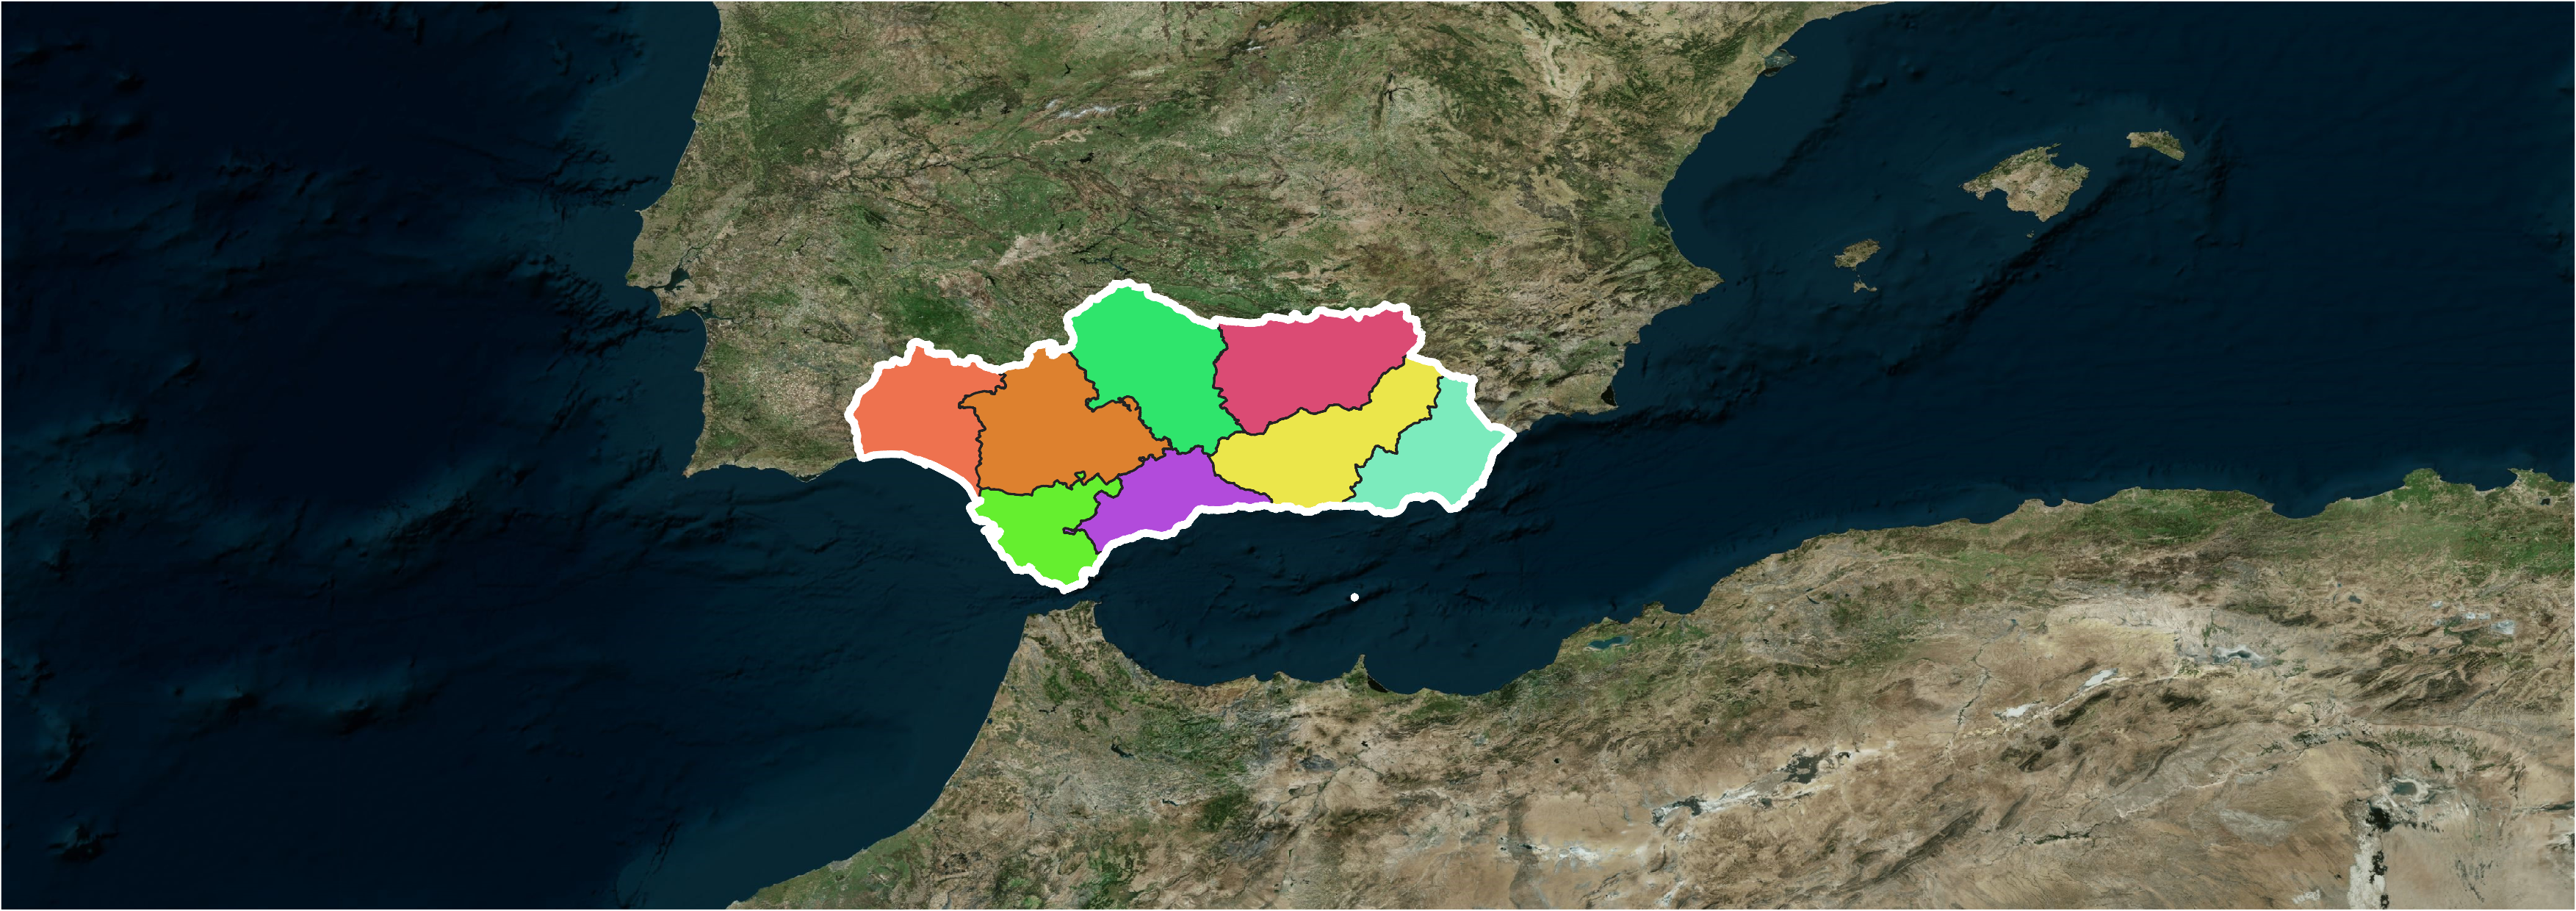
\includegraphics[width=.95\textwidth]{img/provinces_clip_after.png}
			\subcaption{\textit{Después:} Provincias de Andalucía}
		\end{subfigure}
		\caption[Operación de recorte sobre datos geográficos]{Recorte de provincias españolas, delimitado por el polígono de la comunidad andaluza, mostrado como traza en blanco.}
	\end{figure}
	
%	\subsection*{Filtrado por atributos}
	Otra posibilidad es, en vez de utilizar el ámbito geográfico de los datos, usar los datos en sí mismos. Es decir, si consideramos que nuestros datos como una serie de atributos $(x_1, , x_n)$, podemos usar un atributo $x_m$ para filtrar todos aquellos conjuntos que no cumplan las condiciones necesarias para el estudio a desarrollar.
	
	\begin{figure}[htbp]
		\centering
		\includegraphics[width=.6\textwidth]{img/data_filtering.png}
		\caption[Filtrado por atributos específicos]{En este caso de filtrado por atributos, con datos en formato OpenStreetMap, se ha restringido aquellos posibles valores del campo \texttt{highway}, además de eliminado columnas no relevantes, obteniendo un conjunto de datos reducido pero más enfocado al análisis a desarrollar.}
	\end{figure}

	El realizar estas operaciones nos permite eliminar aquellos datos que no sean relevantes a lo que queremos analizar, minimizando el riesgo a error y la carga de procesamiento a realizar.

	\subsection*{Caso Práctico}
	Partiendo de los datos originales a nivel estatal, es decir, de toda España, se ha seleccionado solo aquellos datos que correspondían con carreteras aptas para vehículos motorizados (como coches) en el término municipal de Granada.
	Esto se ha realizado a través de las utilidades de \textit{Osmium}\footnote{Osmium: Proyecto con numerosas herramientas para trabajar con datos de OpenStreetMap. \url{https://osmcode.org/}}.
	
	\begin{minipage}{\textwidth}
	\textbf{\textit{Osmium Extract}} Se ha usado un polígono, descrito en \texttt{GeoJSON}, que corresponde al área municipal de Granada \autocite{GranadaPoly} y se ha invocado de la siguiente forma:
	
	\mint[autogobble,
	frame=single,
%	python3,
%	linenos,
	numbersep=6pt,
	fontsize=\scriptsize,
	bgcolor=mintedbg]{shell}{|>> osmium extract spain-latest.osm.pbf -p granada.json -o granada-latest.osm.pbf}
\end{minipage}

\begin{minipage}{\textwidth}
	\textbf{\textit{Osmium Tags Filter}} Se ha filtrado por todas las primitivas \textsc{Way} cuyo valor de \texttt{highway} comprenda las calles autorizadas para vehículos motorizados, de la siguiente manera:
	\mint[autogobble,
	frame=single,
%	python3,
%	linenos,
	breaklines,
	numbersep=6pt,
	fontsize=\scriptsize,
	bgcolor=mintedbg]{shell}{|>> osmium tags-filter granada-latest.osm.pbf 'w/highway=*_link' 'w/highway=motorway,trunk,primary,secondary,tertiary,residential,living_street' -o granada-latest-highways.osm.pbf}
\end{minipage}

\section{Estructura y Empaquetado}
	Como ya se ha explicado antes, \textit{GeoPackage} es en esencia un contenedor \textit{SQLite}, una base de datos relacional muy portable. Como tal, resulta un formato muy adecuado para datos compuestos por atributos, aunque no necesariamente estén relacionados entre sí.

	\begin{figure}[htbp]
		\centering
		\includegraphics[width=.7\textwidth]{img/network_defn.png}
		\caption[Definición mínima de las entidades de una red]{Como mínimo, debe almacenarse la geometría, y un elemento identificativo, usado para referenciar los nodos en cada enlace, como nodos de origen y de objetivo.}
		\label{network_defn}
	\end{figure}

	Un \textit{GeoPackage} puede estar compuesto por entidades cualesquiera, pero en este caso concreto, necesitaremos dos entidades adicionales, una para nodos y otra para enlaces, tal y como se define en \autoref{network_defn}.
	
	A ambas entidades, como información interesante, se puede añadir una estimación de coste, bien en distancia o tiempo, restricciones de navegabilidad en una u otra dirección, entre otras. Esto se podría hacer directamente en la misma entidad, o en una entidad externa que contenga metadatos y referencie por el identificador
	
	\subsection*{Caso Práctico}
	En el caso práctico, se ha almacenado los datos de Granada, ya procesados y reducidos, sobre un fichero \textit{GeoPackage}. Esto se ha hecho gracias a una herramienta de \textit{GDAL}\footnote{\textit{GDAL/OGR}: Colección de herramientas de software libre para trabajar con datos geográficos. \url{https://gdal.org/}} llamada \textit{ogr2ogr}\footnote{\textit{ogr2ogr}: Herramienta para convertir entre formatos de datos geográficos.}.
	
	\mint[autogobble,
	frame=single,
	python3,
%	linenos,
	numbersep=6pt,
	fontsize=\scriptsize,
	bgcolor=mintedbg]{shell}{|>> osmium extract spain-latest.osm.pbf -p granada.json -o granada-latest.osm.pbf}
	
	Por razones prácticas, no creamos las entidades aún.Esto lo hacemos en el siguiente apartado, directamente con la herramienta que se ha desarrollado para generar la topología.
	
\section{Preparación de la Topología}
	Para generar una topología, tan solo necesitamos todas los enlaces que componen la red a analizar.
	Para crear una topología de dicha red, cada enlace ha de descomponerse en cada intersección entre dos o más enlaces. Para ello, aplicaremos un sencillo algoritmo definido en  \autoref{decompose_ways_algo}.
	
	\begin{listing}[htbp]
		\inputminted[autogobble,
			frame=single,
			python3,
%			linenos,
			numbersep=6pt,
			fontsize=\scriptsize,
			bgcolor=mintedbg,
		]{python}{algorithm_latex.py}
		\caption[Algoritmo para generar una topología]{Dado un conjunto de líneas, para cada línea, dividimos entre dos puntos intermedios, siempre y cuando estos sean válidos, hayan sido usado más de una vez en en el total de las líneas. Como invariante necesaria, se considera que tanto el primer y último punto de una línea son válidos.}
		\label{decompose_ways_algo}
	\end{listing}

	El objetivo de este proceso es la descomposición en unidades únicas, una por cada intersección encontrada a lo largo de una línea. Para llevar esto a cabo, debemos mantener un registro de cuántas veces se utiliza cada punto contenido en cada línea y subdividir cada línea entre dos nodos.
	Una vez tenemos la topología de red procesada, debemos almacenarla en el \textit{GeoPackage} conforme a la estructura descrita en \autoref{network_defn}.
	
	\begin{figure}[htbp]
		\begin{center}
	\begin{subfigure}{0.4\textwidth}
		\centering
		\includegraphics[width=.95\textwidth]{img/topology_before.png}
		\subcaption{Enlaces iniciales}
		\label{topology_before}
	\end{subfigure}
	\begin{subfigure}{0.4\textwidth}
		\centering
		\includegraphics[width=.95\textwidth]{img/topology_after.png}
		\subcaption{Subenlaces resultantes}
		\label{topology_after}
	\end{subfigure}
\end{center}
	\caption[Descomposición topológica de una red]{Descomposición topológica de una red, nótese como cada intersección está delimitada con un redondel. Esto es porque cada enlace se ha dividido en varios enlaces, conservando los lados con varios puntos sin intersección en el proceso.}
	\end{figure}

	
	\subsection*{Caso Práctico}
	Para el caso práctico, se ha desarrollado un software \autocite{gpkgRouting}] en \textit{Python} que utiliza \textit{PyOsmium}\footnote{\textit{PyOsmium}: \textit{Bindings} en Python para la biblioteca \textit{Osmium}} para leer todos las primitivas \textsc{Way} de \textit{OpenStreetMap}. 
	
	\begin{listing}[htbp]
		\inputminted[autogobble,
		frame=single,
		python3,
%		linenos,
		breaklines,
		firstline=52,
		lastline=60,
		numbersep=6pt,
		fontsize=\scriptsize,
		bgcolor=mintedbg,
		]{python}{gpkgrouting/gpkgrouting/handlers.py}
		\caption[Carga de los datos de \textit{OpenStreetMap} con \texttt{gpkgRouting}]{El software carga todos las primitivas \textsc{Way} de un fichero OpenStreetMap y además, para cada elemento, realiza un conteo del número de usos de cada nodo.}
	\end{listing}
	
	Una vez hemos cargados todos los datos, se aplica el algoritmo descrito en \autoref{decompose_ways_algo} para descomponer los caminos en enlaces de una topología y posteriormente almacena la red en un \textit{DataFrame} de \textit{GeoPandas}\footnote{\textit{GeoPandas}: Extensión \textit{GIS} de \textit{Pandas}, \textit{framework} de \textit{Python} con estructuras \textit{DataFrame}, marcos de datos. \url{http://www.geopandas.org/}}, desde la cual exportaremos a GeoPackage. 
	Una vez realizado esto, se almacena el contenido del \textit{DataFrame} en el fichero \textit{GeoPackage} donde tenemos los datos de partida.
	
	\begin{listing}[htbp]
		\inputminted[autogobble,
		frame=single,
		python3,
%		linenos,
		breaklines,
		firstline=108,
		lastline=119,
		numbersep=6pt,
		fontsize=\scriptsize,
		bgcolor=mintedbg,
		]{python}{gpkgrouting/gpkgrouting/handlers.py}
		\caption[Definición de los datos finales obtenidos por \texttt{gpkgRouting}]{Los DataFrame de GeoPandas son una estupenda representación intermedia, ya que son contenedores muy eficientes y además gozan de mucha funcionalidad, como pueda ser directamente exportar a una base de datos \textit{GeoPackage}.}
	\end{listing}
		
	\begin{figure}[htbp]
		\centering
		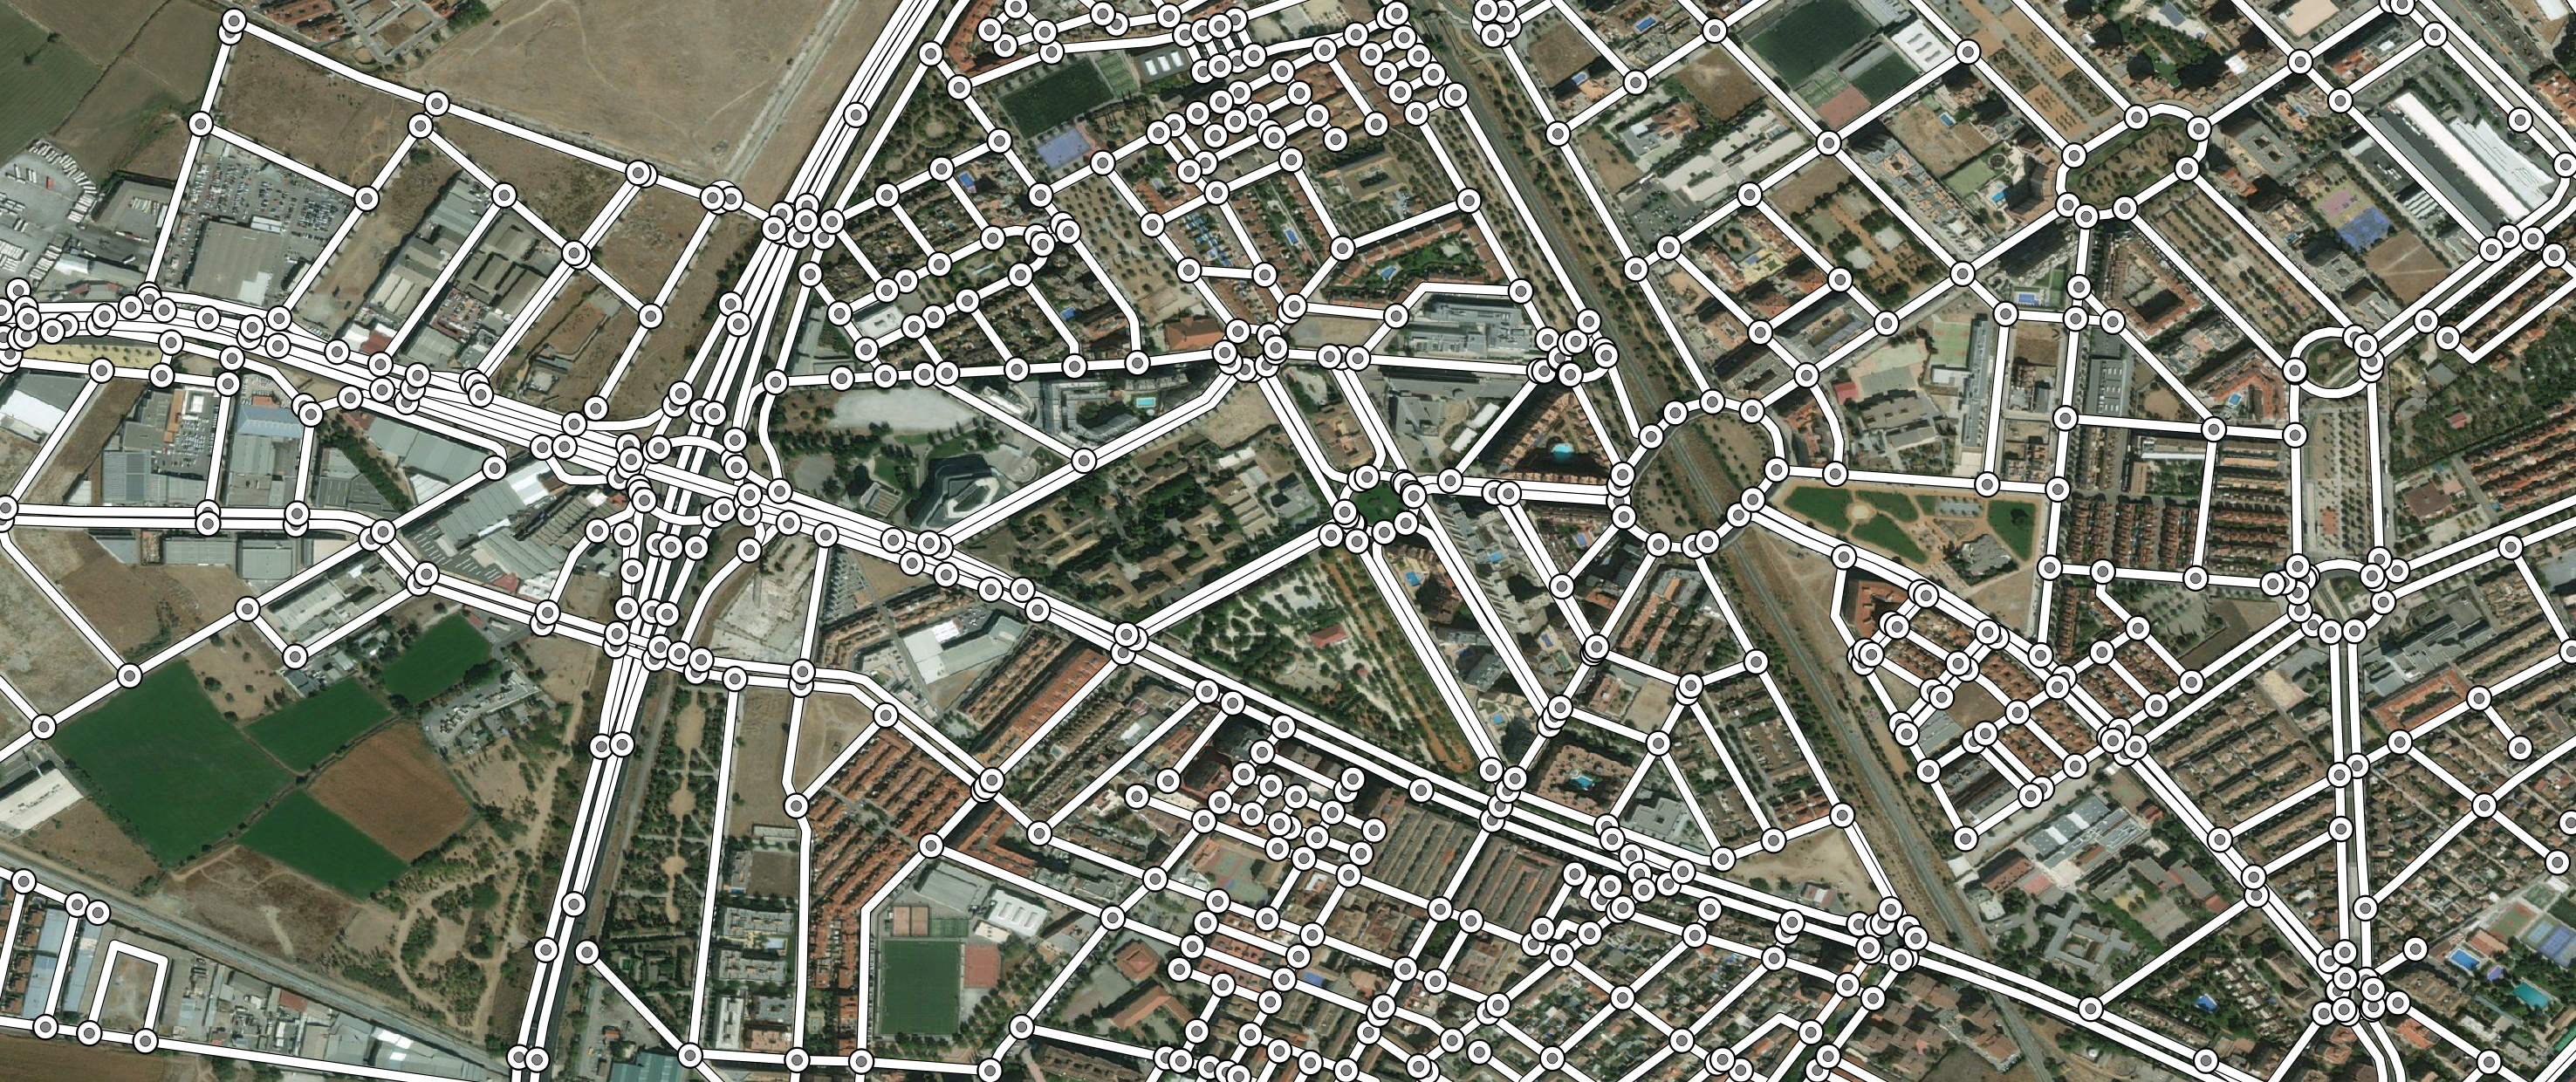
\includegraphics[width=.9\textwidth]{img/granada_topology.png}
		\caption[Topología resultante, visualizada con el software \textit{QGIS}]{Resultado gráfico de la topología resultante al aplicar el software \texttt{gpkgRouting} y visualizado en \textit{QGIS}}
	\end{figure}

\section{Aplicación del Encaminamiento}
	En este momento, tenemos un \textit{GeoPackage} enrutable, el cual podemos inmediatamente utilizar o compartir con terceros como recurso. En el caso de aplicar inmediatamente alguna técnica de encaminamiento, debemos construir un grafo con la información almacenada en nuestro \textit{GeoPackage}.
	
	\begin{figure}[htbp]
		\centering
		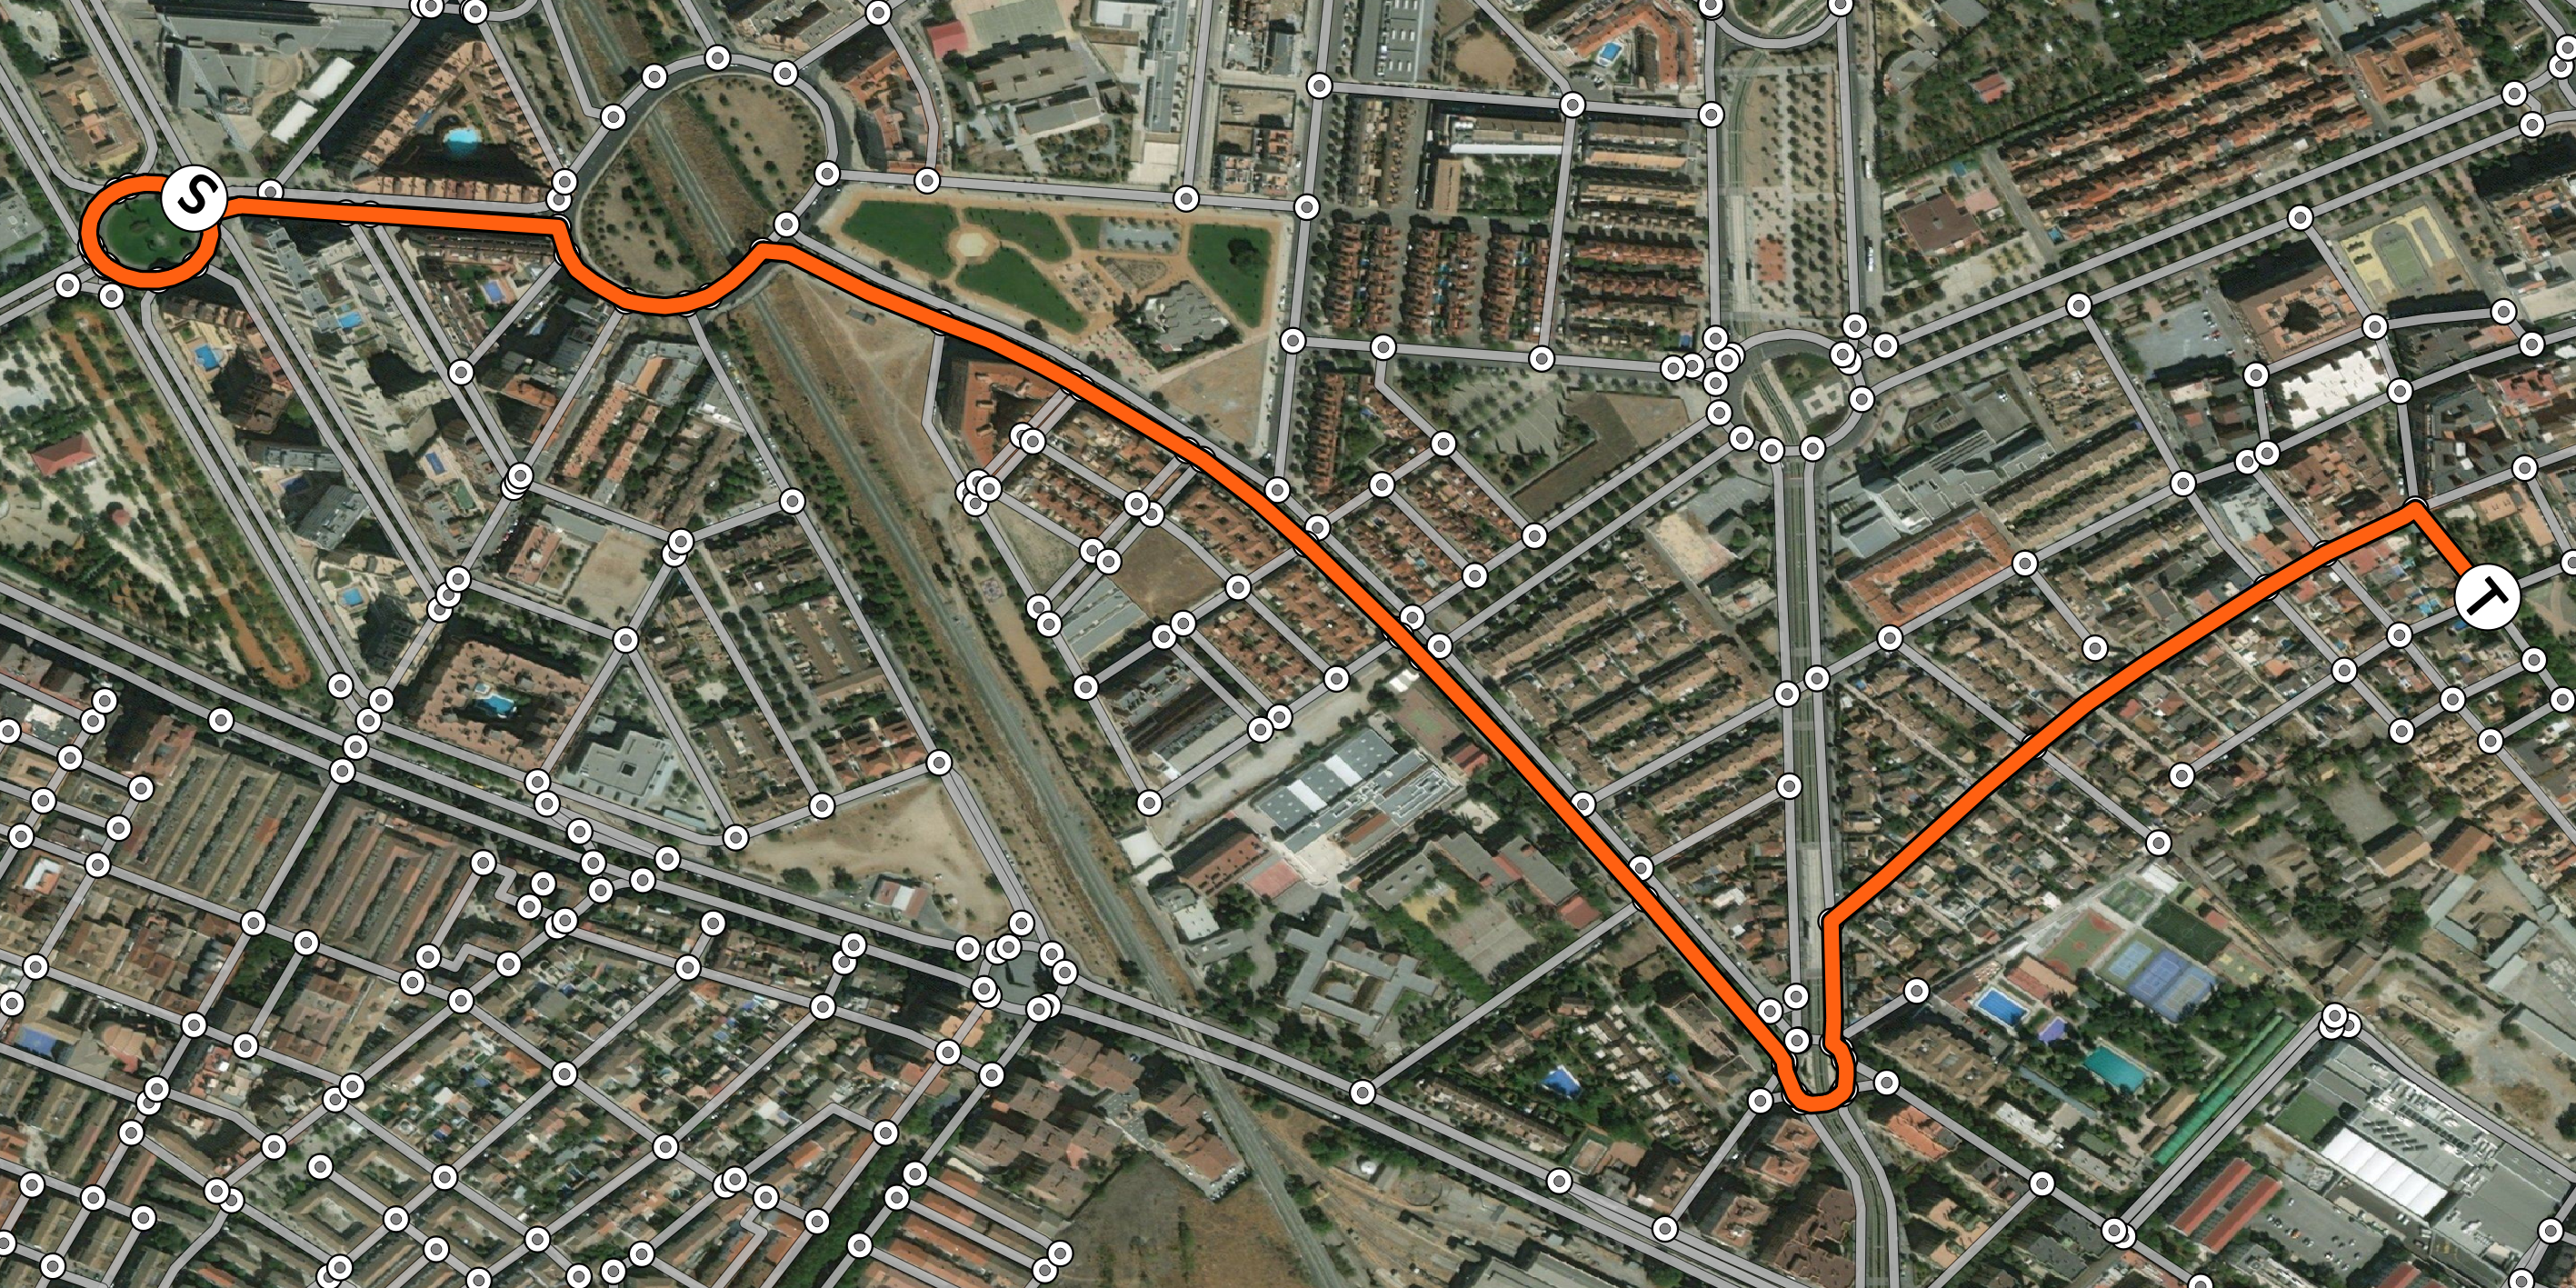
\includegraphics[width=0.78\textwidth]{img/granada_shortest_path}
		\caption[Camino más corto (distancia) entre dos puntos]{Visualizamos el camino obtenido de \autoref{lst:qgis_gpkgrouting} en la suite \textit{QGIS}. En este caso, podemos ver que partimos de ETSIIT y acabamos cerca de la Cámara de Comercio de Granada.}
		\label{pathfinding_granada}
	\end{figure}
	
	Con el grafo ya construido, podremos aplicar algún algoritmo de búsqueda de caminos \autocite[255-287]{gvaliente} para el encaminamiento, existiendo mejores elecciones en función de los datos que tenemos. En el peor caso, siempre podremos aplicar un algoritmo en profundidad usando como coste la distancia de cada enlace.
	
	Heurísticas utilizables podrían ser también el tiempo medio que tarda un vehículo en recorrer una calle, si es que dispusiésemos de tal información. En el caso de haber subdividido un enlace, podríamos considerar la distancia de la división respecto a la distancia total y obtener de ahí un valor proporcional.
	
	\subsection*{Caso Práctico}
	A partir de \textit{NetworkX}\footnote{\textit{NetworkX}: \textit{Framework} de \textit{Python} para tratamiento y operaciones con grafos. \url{https://networkx.github.io/}}, se genera un grafo dirigido en el que todos los enlaces se representan como tuplas $(origen, destino)$ y tienen sus atributos concretos. Con el mismo, se aplican algoritmos como A* para calcular secuencias de nodos por los que pasar para encontrar el camino más óptimo.
	
	\begin{listing}[htbp]
		\begin{minted}[autogobble,
		frame=single,
		python3,
%		linenos,
		breaklines,
		numbersep=6pt,
		fontsize=\scriptsize,
		bgcolor=mintedbg,
		]{python}
		import geopandas as gpd
		import networkx as nx
		df = gpd.from_file('granada-latest-highways.gpkg', driver='GPKG', layer='nw_links')
		G = nx.from_pandas_edgelist(df, create_using=nx.DiGraph)
		
		try:
		path = nx.shortest_path(G, SOURCE, TARGET)
		# Do something with the retrieved path
		...
		except nx.NetworkXNoPath:
		# No path found
		...				
		\end{minted}
		\caption[Encaminamiento con \textit{GeoPackage} y \textit{NetworkX}]{\textit{Python} presenta un ecosistema muy maduro con multitud de herramientas, entre ellas \textit{GeoPandas} y \textit{NetworkX}, que nos permiten trabajar con datos \textit{GIS} y grafos de una forma indolora. Este último, además, tiene funcionalidades de búsqueda de caminos.}
	\end{listing}

\section{Conclusiones}
Dado el análisis y desarrollo llevado a cabo, cabe concluir que es posible almacenar topología en contenedores GeoPackage, y que estos pueden ser usados de forma reiterada para buscar caminos entre nodos de una red.

Es más, al ser un formato relativamente sencillo y casi universalmente aceptado, al ser una base de datos \textit{SQLite}, es trivial profundizar en ámbitos más específicos, que cubran casos de uso concretos. Lo inmediato, y muchas veces mencionado, sería su uso en terminales móviles que, sea por capacidades técnicas o software, no son capaces de aceptar otras soluciones para almacenamiento en local.

Esto, de igual forma, es complejo, ya que no existe un reglamento que enuncie cómo deben estructurarse los datos para que estos sean interpretados de una forma única y correcta, pero por suerte la especificación GeoPackage es abierta y extensible, permitiendo desarrollar extensiones para añadir funcionalidad\footnote{Véase un ejemplo esta extensión titulada \textit{Tiled Gridded Coverage Data Extension}.  \url{http://docs.opengeospatial.org/is/17-066r1/17-066r1.html}}.

Aún así, sea complejo o no, es una posibilidad más para empaquetar y compartir datos geográficos con la oportunidad de realizar consultas de encaminamiento, como herramientas como \textit{pgRouting}. Al fin y al cabo, un ingeniero debe conocer multitud de herramientas o tecnologías para decidir cual es la más conveniente para un problema concreto.
\chapter{Conclusión y Trabajo Futuro}
\label{ch:conclusion}

Como se ha podido comprobar en el capítulo anterior, es muy viable la creación de un \textit{GeoPackage} con información topológica para realizar análisis de redes de carreteras u otro tipo. 

Esto no quiere decir que sea la única ni mejor solución, si no una más, para ámbitos en los que otras soluciones más maduras no puedan implementarse.
De igual manera, sigue siendo una posibilidad más que válida, con un nicho de mercado muy interesante como pueda ser el encaminamiento en local o el empaquetado y envío de datos geográficos enrutables.

Así pues, a continuación se presentan dos secciones, una para desglosar qué objetivos se han cumplido y cómo se ha llevado esto a cabo, y otra para definir qué trabajo futuro podría realizarse sobre las conclusiones resultantes de este análisis.

\section{Objetivos}

Tanto el objetivo principal como los objetivos secundarios han sido completados a lo largo del desarrollo del \textsc{Trabajo de Fin de Grado}. Estos objetivos son listados en la \autoref{sec:objectives}.

El objetivo principal se ha cumplido en toda la realización del \autoref{ch:geopackage_routing}, llevándose a cabo el análisis que se esperaba, obteniendo como conclusiones que sí es viable y las pautas a seguir para obtener un \textit{GeoPackage} enrutable, así como la estructura interna que podrían seguir los datos y algoritmos o extractos de código fuente para completar el proceso.

Los objetivos secundarios se han completado de igual manera, en el proceso de documentación y realización previa a la redacción del documento, y esto se puede observar en el texto y herramientas desarrolladas, a disposición en este mismo documento o en los recursos adicionales presentados al final del mismo.

\begin{itemize}
	\setlength\itemsep{0em}
	\item Se ha conocido la estructura de la base de datos de \textit{OpenStreetMap} a partir de la \textit{OsmWiki}\footnote{Véase \url{https://wiki.openstreetmap.org/wiki/}} y se ha aprendido cómo usar este a partir de la extracción de datos a partir de las herramientas del proyecto \textit{Osmium}.
	
	\item Se han identificado más tipos de contenedores de datos geográficos a través de recursos como sean \autocite{volaya} o \autocite{bolstad} y qué ventajas o desventajas presentan.
	
	\item Se ha encontrado herramientas como \textit{Osmium}, \textit{GeoPandas}, \textit{NetworkX}, entre otras, para la creación, manipulación y visualización de datos geográficos en un entorno general.
	
	\item Referente al punto anterior, muchas herramientas anteriormente citadas funcionan bajo un entorno \textsc{Python}, o tienen algún tipo de \textit{binding}, así pues se exhibe que dicho entorno es muy capaz a la hora de trabajar con información geográfica y análisis estadísticos o de otro tipo.
\end{itemize}

\section{Trabajo Futuro}
El trabajo, una vez finalizado y con sus conclusiones presentadas, podría llegar a extenderse por varios caminos.

Por un lado, se podría ver la posibilidad de la estandarización del modelo de representación de componentes topológicas, la propia red de conexiones entre nodos y los nodos en sí, como una extensión del estándar \textit{GeoPackage}. De esto llevarse a cabo, habría que producir un boceto técnico y presentarse al \textit{Open Geospatial Consortium} como una extensión de la comunidad\footnote{Véase \url{https://www.geopackage.org/extensions.html}}. Una vez esto, debería ser publicitado, implementado y revisado reiteradamente hasta que finalmente acepte la madurez necesaria para que se convierta en una extensión oficial.

Por otro lado, cabe la posibilidad de extender la prueba de concepto desarrollada, añadiendo mayor cantidad de funcionalidades aunque dependa internamente de los mismos proyectos ya comentados, llámese \textit{NetworkX}, \textit{GeoPandas}, \textit{Osmium}, además de otros. El objetivo principal de este proyecto debería ser la accesibilidad a desarrolladores, así pues siendo un nexo de enlace entre las muchas herramientas ya comentadas.

Otra posibilidad relacionada con la anterior, sería utilizar las herramientas de más bajo nivel, fuera del ecosistema \textsc{Python}, y buscar herramientas más portables a otras plataformas, como pueda ser basadas en tecnologías como \textsc{C++} o \textsc{Java}, idealmente con el mismo planteamiento que la propuesta anterior, la accesibilidad a otros desarrolladores.

Este trabajo también puede, propiamente dicho, ayudarme a encontrar trabajo en el sector \textit{GIS}, donde podría plasmar todo el conocimiento adquirido y refinado en la elaboración del análisis y de la misma implementación.
\appendix
\chapter{Planificación del Proyecto}\label{app:planification}

Aunque no se ha llevado ninguna metodología concreta como podría ser, por ejemplo, \textit{Scrum}, se aplicado una metodología ágil e incremental al realizarse prototipos o bocetos sobre los que se ha continuado el desarrollo, también con gran cantidad de realimentación al solicitar opinión a mi tutor, José Samos Jiménez, tanto por correo como en horario de tutorías.

Dicho esto y considerando que, en España, un crédito \textit{ECTS} equivale a 25 horas de estudio, y que la asignatura de \textsc{Trabajo de Fin de Grado} se compone de 12 créditos \textit{ECTS}, el tiempo a dedicar a este trabajo debería haber sido 240 horas, el cual se ha desarrollado por fases descritas en \autoref{tab:planification}. Este tiempo ha sido alcanzado e incluso superado, por dedicarle horas en las que no conseguía un rendimiento muy alto. 

Este trabajo se ha desglosado por actividades en las proporciones que se muestran en \autoref{tab:planification_tasks}.

\begin{table}[htbp]
	\centering
	\begin{tabular}{r || l | c  c }
		\textbf{Período} & \textbf{Enfoque} & \textbf{Tiempo} & \textbf{Dedicación} \\
		\hline\hline
		\textbf{Primer Semestre} & Estudio e Investigación & 36 horas & 15\% \\
		\textbf{Segundo Semestre} & Experimentar y Codificar & 72 horas & 30\%\\
		\textbf{Período de Verano} & Desarrollo del Documento & 132 horas & 55\%\\
		\hline
		& Trabajo de Fin de Grado & 240 horas & 100\%
	\end{tabular}
	\caption[Planificación general del proyecto]{El esfuerzo se ha repartido a lo largo del periodo académico comprendido entre los años dos mil dieciocho y diecinueve (\textsc{2018-2019}), en una proporción irregular, por cuestiones de tiempo disponible.}
	\label{tab:planification}
\end{table}

\begin{table}[htbp]
	\centering
	\begin{tabular}{ r ||l | c c}
		\textbf{Período} & \textbf{Actividad} & \textbf{Tiempo} & \textbf{Dedicación} \\
		\hline\hline
		\textbf{I} & Estudio de Herramientas & 18 horas & 7.5\% \\
		\textbf{I} & Análisis de Viabilidad & 18 horas & 7.5\% \\
		\textbf{II} & Diseño del Software & 36 horas & 15\% \\
		\textbf{II} & Codificación del Software & 36 horas & 15\% \\
		\textbf{III} & Desarrollo del Documento & 120 horas & 50\% \\
		\textbf{III} & Incorporación en otras Soluciones & 6 horas & 2.5\% \\
		\textbf{III} & Creación de Recursos Gráficos & 6 horas & 2.5\%\\
		\hline
		 & Trabajo de Fin de Grado & 240 horas & 100\%
	\end{tabular}
	\caption[Planificación por actividad]{El desarrollo de cada actividad ha estado realmente intercalado con otras actividades, por ejemplo la creación de recursos gráficos se ha llevado a cabo durante la realización del documento. Los tiempos y porcentajes dados son estimaciones de la realidad.}
	\label{tab:planification_tasks}
\end{table}

\section*{Explicación}
Elegí desarrollar y exponer este trabajo en un año, académicamente, muy pesado al estar cursando once asignaturas además de este trabajo, completando un total de 78 créditos \textit{ECTS}.

Como tal, el proyecto partió de una planificación rígida a algo más flexible. Quise partir de repartir mi tiempo a partes iguales en investigar, desarrollar y escribir. Esto, como cabía esperar, no se cumplió y acabó siendo diferente, véase \autoref{tab:planification}.

Como tal, empecé en el primer semestre del año académico buscando ideas sobre qué desarrollar como objeto de mi \textsc{Trabajo de Fin de Grado}. En la susodicha asignatura de \textsc{Sistemas de Información Geográficos} elegí el tema a tratar, por mi cariño a la asignatura y mi interés en una tecnología libre como \textit{GeoPackage}.

Ese semestre no logré mucho más que aprender sobre \textit{GIS} y diseñar ciertos prototipos, como la inyección de funciones \textit{SQL} para imitar a \textit{pgRouting}, pero por limitaciones de \textit{SQLite}, tuve que desestimarlo.

Al siguiente, segundo semestre, logré desarrollar más el texto, particularmente la estructura y los elementos a introducir, pero la ausencia de tiempo me hizo dejar la entrega final a Septiembre.

En los meses de verano, ya con todo o gran parte del código desarrollado y la idea bien clara, he dedicado gran parte de mi tiempo diario a el desarrollo del documento, sea texto o recursos como figuras o códigos.

Consolidando toda esta información explicada arriba, podríamos decir que este proyecto se ha desarrollado en tres fases, primer y segundo semestre académico y los meses de verano, cada uno con un enfoque y una dedicación concreta.
\chapter{Integración con \textit{QGIS}}
\label{app:qgis_integration}

\textit{QGIS}, una herramienta \textit{GIS} de software libre muy capaz y multiplataforma, cuenta tanto con un sistema de \textit{plugins} como con un entorno de consola, ambas con soporte para \textsc{Python} y su ecosistema. Por tanto, integrar la prueba de concepto con \textit{QGIS} es casi inmediato, ya que todo lo desarrollado usa \textsc{Python} como forma de implementación.

En el siguiente ejemplo \autoref{lst:qgis_gpkgrouting}, se carga un fichero \textit{GeoPackage} ya enrutable, obtenido a través del proceso descrito en el capítulo \textsc{Encaminamiento con GeoPackage}, se genera un grafo y se realizan consultas de encaminamiento sobre este. Concretamente, el ejemplo mostrado es aquel que genera la imagen mostrada en \autoref{pathfinding_granada}.

Por ser una mera prueba de concepto, se trata de un simple \textit{script} y no es un \textit{plugin} como tal, ya que existen otra herramientas que te ofrecen una herramienta similar dentro de \textit{QGIS}, como las extensiones de \textit{GRASS}.

\begin{listing}[htbp]
	\inputminted[autogobble,
	frame=single,
	python3,
	linenos,
	numbersep=6pt,
	fontsize=\scriptsize,
	bgcolor=mintedbg,
	]{python}{qgis/qgis_gpkgrouting.py}
	\caption[Integración con QGIS]{qgis\_gpkgrouting.py}
	\label{lst:qgis_gpkgrouting}
\end{listing}
\printbibliography[heading=bibintoc, title={Bibliografía y Referencias}, category=cited, nottype=online]
\printbibliography[heading=subbibintoc, title={Lectura Adicional},  notcategory=cited, nottype=online]
\printbibliography[heading=subbibintoc, title={Recursos Electrónicos}, type=online]

\end{document}
